\documentclass[../ClipsManualeUtente.tex]{subfiles}

\begin{document}
\section{Installazione}
	Di seguito si elencano i passaggi necessari per la corretta installazione dell'applicazione nello smartphone.
	

		\subsection{Download applicazione}
			\begin{enumerate}
				\item Dal proprio smartphone aprire il browser preferito;
				\item digitare correttamente il seguente indirizzo web: \\
					\url{http://leafswe.github.io/download/};
				\item premere il pulsante \textbf{download} come in figura \ref{fig:DownloadApplicazioneSito};
				\item accettare il download.
			\end{enumerate}
			
			\begin{figure} [h]
				\centering
				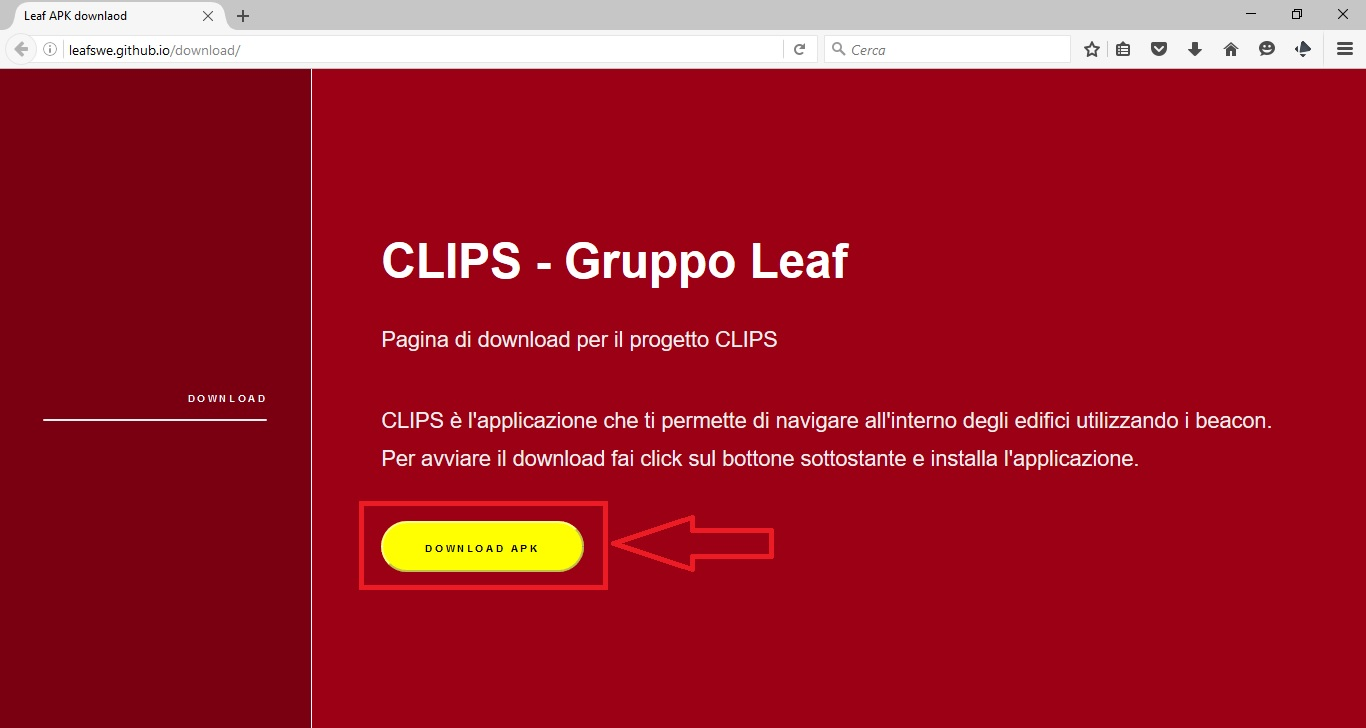
\includegraphics[width=\textwidth]{img/DownloadApplicazioneSito}
				\caption{Pagina del sito da cui effettuare il download dell'applicazione}
				\label{fig:DownloadApplicazioneSito}
			\end{figure}
		
		\newpage
		\subsection{Sblocco controlli di sicurezza per installare l'applicazione}
		
			\begin{framed}
				\textbf{Nota:} l'applicazione è sperimentale per cui il procedimento per l'installazione non è agevolato da nessun \gls{Marketplace} (per esempio \gls{Google} Play) e necessita di passaggi in più rispetto all'installazione di una normale applicazione.
			\end{framed}
		
			\begin{enumerate}
				\item Selezionare il file \verb|app-debug.apk| scaricato;
				\item il sistema ti avviserà che l'installazione è bloccata per applicazioni con fonti non certificate (figura \ref{fig:InstallazioneBloccata}). Premi \textit{Impostazioni} per andare nelle impostazioni del tuo smartphone;
				
				\begin{figure}[h]
					\centering
					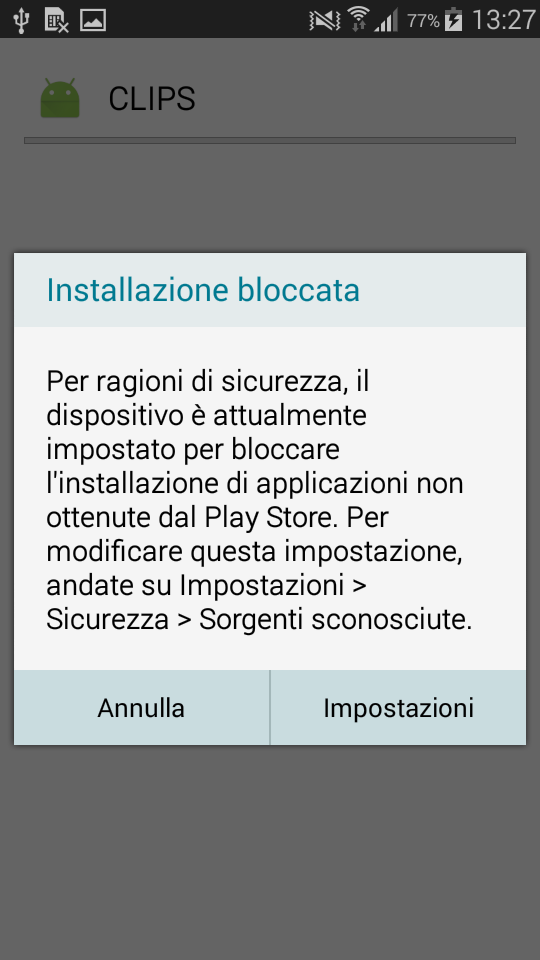
\includegraphics[scale=0.25]{img/InstallazioneBloccata}
					\caption{Avviso del sistema per l'installazione di applicazioni non certificate}
					\label{fig:InstallazioneBloccata}
				\end{figure}
				
				\item dalla schermata \textit{Sicurezza} aperta seleziona \textit{Sorgenti sconosciute} come in figura \ref{fig:ImpostazioniPermessi};
				\item nella finestra di dialogo aperta (figura \ref{fig:SorgentiSconosciute}) selezionare \textit{OK}.
				\end{enumerate}	
				
				\begin{figure} [h]
					\centering
					\subfloat[][Schermata delle impostazioni di sicurezza del proprio smartphone]
					{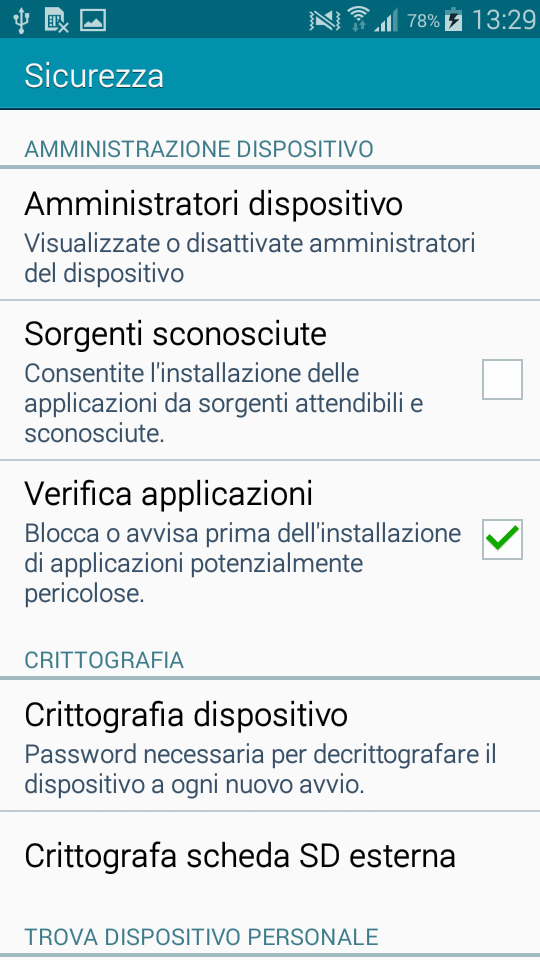
\includegraphics[width=.33\textwidth]{img/ImpostazioniPermessi}
					\label{fig:ImpostazioniPermessi}} \quad
					\hspace{1.5cm}
					\subfloat[][Finestra di accettazione installazione di applicazioni da sorgenti sconosciute]
					{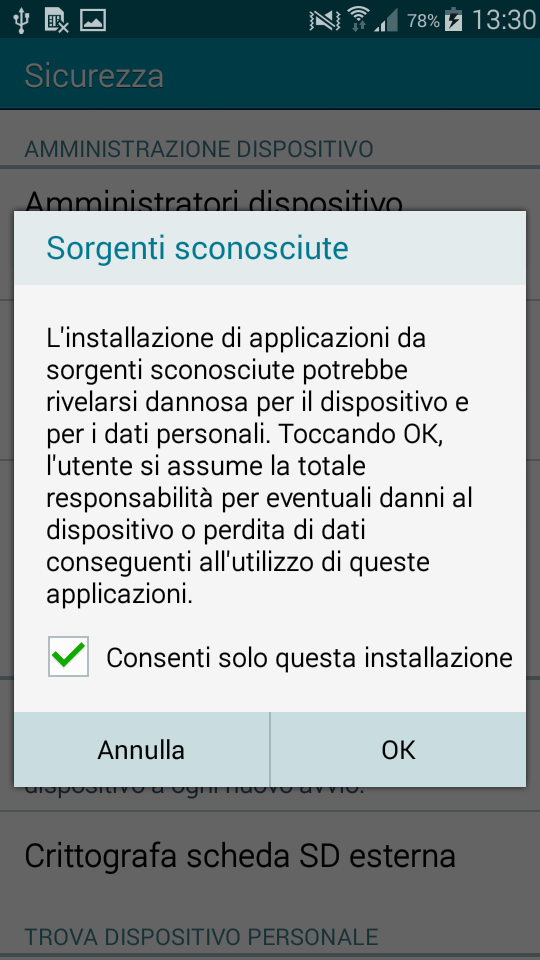
\includegraphics[width=.33\textwidth]{img/SorgentiSconosciute}
					\label{fig:SorgentiSconosciute}} \\
					
					%\caption{}
					%\label{fig:Sicurezza}
				\end{figure}				
				
		\newpage
		\subsection{Installazione applicazione}		
		
		\begin{enumerate}
			\item Selezionare \textbf{Installa} e accettare che l'applicazione sia installata nel proprio dispositivo.
		\end{enumerate}
		
			\vfill
			\begin{figure} [h]
				\centering
				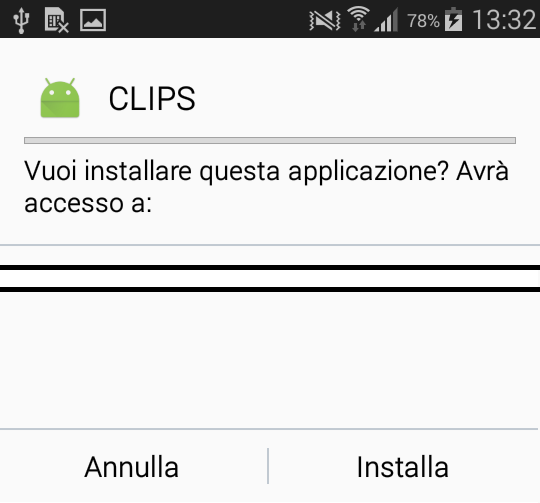
\includegraphics[scale=0.3]{img/Installa_}
				\caption{Schermata di installazione dell'applicazione}
				\label{fig:Installa}
			\end{figure}
			\vfill
		
		
\end{document}